% Options for packages loaded elsewhere
\PassOptionsToPackage{unicode}{hyperref}
\PassOptionsToPackage{hyphens}{url}
%
\documentclass[
]{book}
\usepackage{amsmath,amssymb}
\usepackage{iftex}
\ifPDFTeX
  \usepackage[T1]{fontenc}
  \usepackage[utf8]{inputenc}
  \usepackage{textcomp} % provide euro and other symbols
\else % if luatex or xetex
  \usepackage{unicode-math} % this also loads fontspec
  \defaultfontfeatures{Scale=MatchLowercase}
  \defaultfontfeatures[\rmfamily]{Ligatures=TeX,Scale=1}
\fi
\usepackage{lmodern}
\ifPDFTeX\else
  % xetex/luatex font selection
\fi
% Use upquote if available, for straight quotes in verbatim environments
\IfFileExists{upquote.sty}{\usepackage{upquote}}{}
\IfFileExists{microtype.sty}{% use microtype if available
  \usepackage[]{microtype}
  \UseMicrotypeSet[protrusion]{basicmath} % disable protrusion for tt fonts
}{}
\makeatletter
\@ifundefined{KOMAClassName}{% if non-KOMA class
  \IfFileExists{parskip.sty}{%
    \usepackage{parskip}
  }{% else
    \setlength{\parindent}{0pt}
    \setlength{\parskip}{6pt plus 2pt minus 1pt}}
}{% if KOMA class
  \KOMAoptions{parskip=half}}
\makeatother
\usepackage{xcolor}
\usepackage{color}
\usepackage{fancyvrb}
\newcommand{\VerbBar}{|}
\newcommand{\VERB}{\Verb[commandchars=\\\{\}]}
\DefineVerbatimEnvironment{Highlighting}{Verbatim}{commandchars=\\\{\}}
% Add ',fontsize=\small' for more characters per line
\usepackage{framed}
\definecolor{shadecolor}{RGB}{248,248,248}
\newenvironment{Shaded}{\begin{snugshade}}{\end{snugshade}}
\newcommand{\AlertTok}[1]{\textcolor[rgb]{0.94,0.16,0.16}{#1}}
\newcommand{\AnnotationTok}[1]{\textcolor[rgb]{0.56,0.35,0.01}{\textbf{\textit{#1}}}}
\newcommand{\AttributeTok}[1]{\textcolor[rgb]{0.13,0.29,0.53}{#1}}
\newcommand{\BaseNTok}[1]{\textcolor[rgb]{0.00,0.00,0.81}{#1}}
\newcommand{\BuiltInTok}[1]{#1}
\newcommand{\CharTok}[1]{\textcolor[rgb]{0.31,0.60,0.02}{#1}}
\newcommand{\CommentTok}[1]{\textcolor[rgb]{0.56,0.35,0.01}{\textit{#1}}}
\newcommand{\CommentVarTok}[1]{\textcolor[rgb]{0.56,0.35,0.01}{\textbf{\textit{#1}}}}
\newcommand{\ConstantTok}[1]{\textcolor[rgb]{0.56,0.35,0.01}{#1}}
\newcommand{\ControlFlowTok}[1]{\textcolor[rgb]{0.13,0.29,0.53}{\textbf{#1}}}
\newcommand{\DataTypeTok}[1]{\textcolor[rgb]{0.13,0.29,0.53}{#1}}
\newcommand{\DecValTok}[1]{\textcolor[rgb]{0.00,0.00,0.81}{#1}}
\newcommand{\DocumentationTok}[1]{\textcolor[rgb]{0.56,0.35,0.01}{\textbf{\textit{#1}}}}
\newcommand{\ErrorTok}[1]{\textcolor[rgb]{0.64,0.00,0.00}{\textbf{#1}}}
\newcommand{\ExtensionTok}[1]{#1}
\newcommand{\FloatTok}[1]{\textcolor[rgb]{0.00,0.00,0.81}{#1}}
\newcommand{\FunctionTok}[1]{\textcolor[rgb]{0.13,0.29,0.53}{\textbf{#1}}}
\newcommand{\ImportTok}[1]{#1}
\newcommand{\InformationTok}[1]{\textcolor[rgb]{0.56,0.35,0.01}{\textbf{\textit{#1}}}}
\newcommand{\KeywordTok}[1]{\textcolor[rgb]{0.13,0.29,0.53}{\textbf{#1}}}
\newcommand{\NormalTok}[1]{#1}
\newcommand{\OperatorTok}[1]{\textcolor[rgb]{0.81,0.36,0.00}{\textbf{#1}}}
\newcommand{\OtherTok}[1]{\textcolor[rgb]{0.56,0.35,0.01}{#1}}
\newcommand{\PreprocessorTok}[1]{\textcolor[rgb]{0.56,0.35,0.01}{\textit{#1}}}
\newcommand{\RegionMarkerTok}[1]{#1}
\newcommand{\SpecialCharTok}[1]{\textcolor[rgb]{0.81,0.36,0.00}{\textbf{#1}}}
\newcommand{\SpecialStringTok}[1]{\textcolor[rgb]{0.31,0.60,0.02}{#1}}
\newcommand{\StringTok}[1]{\textcolor[rgb]{0.31,0.60,0.02}{#1}}
\newcommand{\VariableTok}[1]{\textcolor[rgb]{0.00,0.00,0.00}{#1}}
\newcommand{\VerbatimStringTok}[1]{\textcolor[rgb]{0.31,0.60,0.02}{#1}}
\newcommand{\WarningTok}[1]{\textcolor[rgb]{0.56,0.35,0.01}{\textbf{\textit{#1}}}}
\usepackage{longtable,booktabs,array}
\usepackage{calc} % for calculating minipage widths
% Correct order of tables after \paragraph or \subparagraph
\usepackage{etoolbox}
\makeatletter
\patchcmd\longtable{\par}{\if@noskipsec\mbox{}\fi\par}{}{}
\makeatother
% Allow footnotes in longtable head/foot
\IfFileExists{footnotehyper.sty}{\usepackage{footnotehyper}}{\usepackage{footnote}}
\makesavenoteenv{longtable}
\usepackage{graphicx}
\makeatletter
\def\maxwidth{\ifdim\Gin@nat@width>\linewidth\linewidth\else\Gin@nat@width\fi}
\def\maxheight{\ifdim\Gin@nat@height>\textheight\textheight\else\Gin@nat@height\fi}
\makeatother
% Scale images if necessary, so that they will not overflow the page
% margins by default, and it is still possible to overwrite the defaults
% using explicit options in \includegraphics[width, height, ...]{}
\setkeys{Gin}{width=\maxwidth,height=\maxheight,keepaspectratio}
% Set default figure placement to htbp
\makeatletter
\def\fps@figure{htbp}
\makeatother
\setlength{\emergencystretch}{3em} % prevent overfull lines
\providecommand{\tightlist}{%
  \setlength{\itemsep}{0pt}\setlength{\parskip}{0pt}}
\setcounter{secnumdepth}{5}
\usepackage{booktabs}
\ifLuaTeX
  \usepackage{selnolig}  % disable illegal ligatures
\fi
\usepackage[]{natbib}
\bibliographystyle{plainnat}
\usepackage{bookmark}
\IfFileExists{xurl.sty}{\usepackage{xurl}}{} % add URL line breaks if available
\urlstyle{same}
\hypersetup{
  pdftitle={Guide R},
  pdfauthor={Mégane Bollenrücher},
  hidelinks,
  pdfcreator={LaTeX via pandoc}}

\title{Guide R}
\author{Mégane Bollenrücher}
\date{2025-02-11}

\begin{document}
\maketitle

{
\setcounter{tocdepth}{1}
\tableofcontents
}
Merci de prendre note que ce bookdown est en cours de rédaction.

\chapter{Introduction}\label{introduction}

Ceci est le guide R que nous proposons pour vous accompagner durant les travaux pratiques de méthodologique.

\chapter{Installation et environnement R et Rstudio}\label{installation-et-environnement-r-et-rstudio}

\section{Présentation des logiciels}\label{pruxe9sentation-des-logiciels}

R est un langage de programmation adapté au traitement de données et à l'analyse statistique.

Pour programmer en langage R, il est nécessaire d'installer deux outils essentiels:

\begin{enumerate}
\def\labelenumi{\arabic{enumi}.}
\tightlist
\item
  Le \textbf{logiciel R} permet de traduire du texte sous forme de code R en binaire qui est le langage interne du processeur de l'ordinateur.
\item
  Le \textbf{logiciel RStudio} permet de faciliter l'utilisation du logiciel R en donnant l'accès à une interface utilisateur.
\end{enumerate}

Il est possible de faire une analogie avec une voiture. Le logiciel R est le moteur et RStudio est le tableau de bord. Sans le tableau de bord, il n'est pas possible de controler le moteur.

\section{Installation}\label{installation}

\begin{enumerate}
\def\labelenumi{\arabic{enumi}.}
\tightlist
\item
  Installer R sur le site de R.

  \begin{enumerate}
  \def\labelenumii{\roman{enumii}.}
  \tightlist
  \item
    Choisir et télécharger la version de R selon votre système d'exploitation.

    \begin{itemize}
    \tightlist
    \item
      Pour windows : \url{https://cran.r-project.org/bin/windows/base/}
    \item
      Pour MAC : \url{https://cran.r-project.org/bin/macosx/}
    \item
      Pour Linux : \url{https://cran.r-project.org/index.html}
    \end{itemize}
  \item
    Installer le logiciel R sur votre ordinateur en exécutant le fichier téléchargé.
  \end{enumerate}
\item
  Installer RStudio sur le site suivant: \url{https://posit.co/download/rstudio-desktop/}
\end{enumerate}

Après avoir installé ces deux logiciels, vous aurez accès à deux nouvelles applications. Cependant, nous utiliserons uniquement RStudio pour programmer. Lorsque vous exécuterez votre code écrit sur RStudio, ce dernier fera automatiquement appel à R pour exécuter les codes.

\section{Environnement de travail}\label{environnement-de-travail}

Une fois que RStudio est lancé, une interface découpée en plusieurs zones se présente. Ces parties parties peuvent être redimensionnées, masquées ou maximisées selon vos préférences.

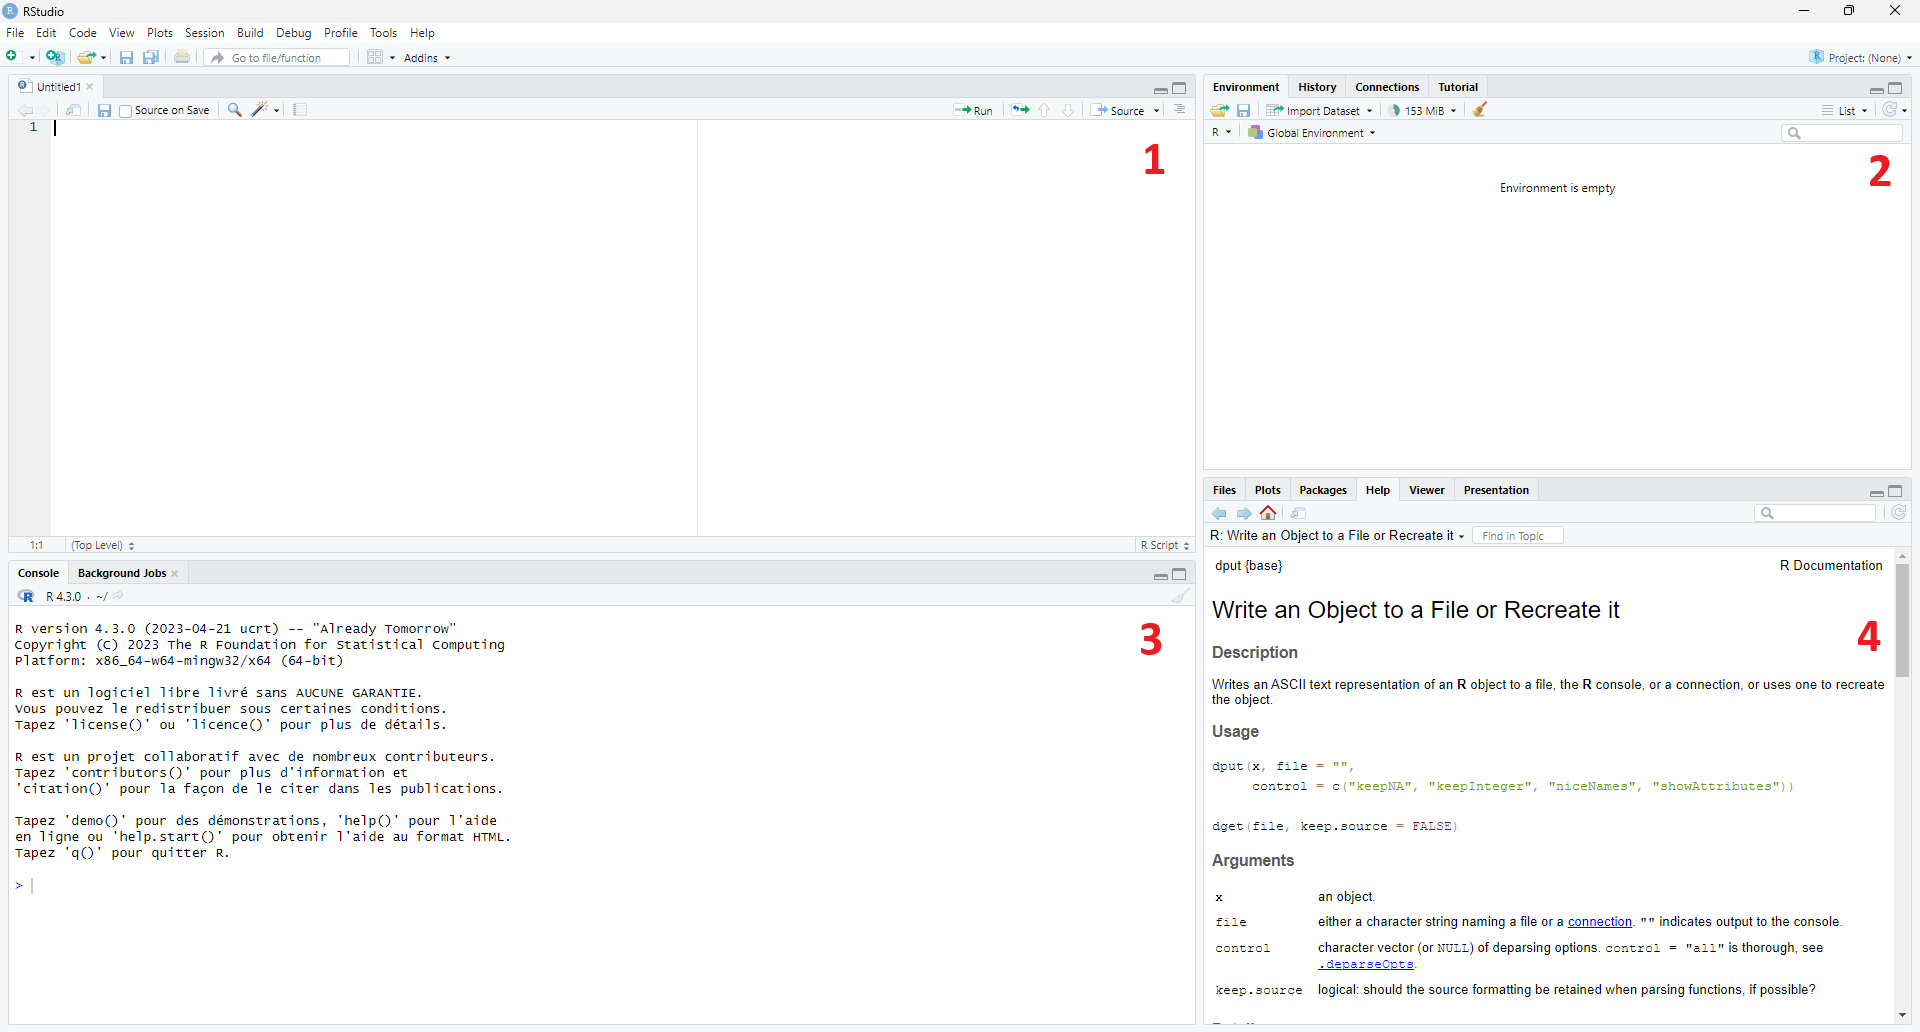
\includegraphics[width=26.67in]{images/environnement}
Chacune des quatre zones a sa propre utilité:

\begin{enumerate}
\def\labelenumi{\arabic{enumi}.}
\tightlist
\item
  Cette zone est dédiée aux fichiers sources. Ce volet permet d'écrire et de sauvegarder les lignes de code. Ce sera la partie la plus utilisée lors de la programmation. Un nouveau script peut être ouvert à partir de l'onglet \texttt{File} en haut à gauche de l'écran, puis \texttt{New\ File} et \texttt{R\ Script}. Chaque script peut être enregistré soit via le même onglet en choisissant \texttt{Save\ As}, soit en utilisant les raccourcis classiques de votre clavier.
\item
  Cette zone fournit des informations sur les objets, les variables et les données en mémoire sous l'onglet \texttt{Environment}.
\item
  La console est affichée en bas à gauche. Cette partie permet d'entrer et d'exécuter des instructions et voir les résultats s'afficher.
\item
  Cette zone permet de naviguer dans le répertoire de travail dans l'onglet \texttt{Files}, d'afficher les graphes réalisés dans l'onglet \texttt{Plots}, d'afficher les extensions/packages disponibles sous l'onglet \texttt{Packages} et également d'afficher l'aide (qui est très complète) sous l'onglet \texttt{Help}.
\end{enumerate}

\chapter{Objets et opérateurs}\label{objets-et-opuxe9rateurs}

\section{Objets dans R}\label{objets-dans-r}

Une variable permet de stocker une valeur ou un objet dans R. De cette façon, il sera possible d'accéder à la valeur ou à l'objet qui est stocké dans la variable.

\begin{Shaded}
\begin{Highlighting}[]
\CommentTok{\# Assignation de la valeur 3 à la variable "ma\_variable"}
\NormalTok{ma\_variable }\OtherTok{\textless{}{-}} \DecValTok{3}
\end{Highlighting}
\end{Shaded}

La ligne de code ci-dessus déclare une variable nommée ``ma\_variable'' et lui assigne la valeur de 3. L'exécution de ce code n'affiche pas de résultat dans la console, mais l'objet nommé ``ma\_variable'' est bien créée et stockée dans l'environnement.

Pour afficher le contenu de la variable, il suffit de taper le nom de celle-ci pour l'afficher dans la console.

\begin{Shaded}
\begin{Highlighting}[]
\CommentTok{\# Affichage du contenu de la variable "ma\_variable"}
\NormalTok{ma\_variable}
\end{Highlighting}
\end{Shaded}

\begin{verbatim}
## [1] 3
\end{verbatim}

De plus, il est également possible d'utiliser la fonction \texttt{print()} qui permet d'afficher la valeur ou l'objet de la variable sélectionnée.

\begin{Shaded}
\begin{Highlighting}[]
\CommentTok{\# Affichage du contenur de la variable "ma\_variable"}
\FunctionTok{print}\NormalTok{(ma\_variable)}
\end{Highlighting}
\end{Shaded}

\begin{verbatim}
## [1] 3
\end{verbatim}

En langage R, il existe différents types d'objets qui peuvent être assignés à des variables comme les scalaires, les vecteurs, les facteurs, les matrices et les bases de données. Ces objets sont présentés dans les points suivants.

\subsection{Scalaire}\label{scalaire}

Un scalaire permet de stocker un objet sous forme de valeur numérique, de chaîne de caractères ou de valeur logique.

\begin{Shaded}
\begin{Highlighting}[]
\CommentTok{\# Scalaire numerique}
\NormalTok{a }\OtherTok{\textless{}{-}} \DecValTok{3}
\NormalTok{a}
\end{Highlighting}
\end{Shaded}

\begin{verbatim}
## [1] 3
\end{verbatim}

Une chaîne de caractères est une suite de caractères qui doit être écrit entre guillemets ('' ``).

\begin{Shaded}
\begin{Highlighting}[]
\CommentTok{\# Scalaire sous forme d\textquotesingle{}une chaine de caractères}
\NormalTok{b }\OtherTok{\textless{}{-}} \StringTok{"Statistique"}
\NormalTok{b}
\end{Highlighting}
\end{Shaded}

\begin{verbatim}
## [1] "Statistique"
\end{verbatim}

Une valeur logique est une quantitée binaire (vrai ou faux). Ces variables s'écrivent \texttt{TRUE} et \texttt{FALSE}. Il est également possible d'utiliser \texttt{T} et \texttt{F} comme abréviations.

\begin{Shaded}
\begin{Highlighting}[]
\CommentTok{\# Scalaire logique}
\NormalTok{c }\OtherTok{\textless{}{-}} \ConstantTok{TRUE}
\NormalTok{c}
\end{Highlighting}
\end{Shaded}

\begin{verbatim}
## [1] TRUE
\end{verbatim}

\begin{Shaded}
\begin{Highlighting}[]
\NormalTok{d }\OtherTok{\textless{}{-}}\NormalTok{ F}
\NormalTok{d  }
\end{Highlighting}
\end{Shaded}

\begin{verbatim}
## [1] FALSE
\end{verbatim}

\subsection{Vecteur}\label{vecteur}

Un vecteur est un objet qui permet de stocker une liste ordonnée d'éléments. Les éléments d'un vecteur doivent être du même type.
Pour pouvoir stocker une information dans un seul objet, il faut utiliser la fonction \texttt{c()} qui permet de combiner les arguments de la fonction.

\begin{Shaded}
\begin{Highlighting}[]
\CommentTok{\# Vecteur numérique}
\NormalTok{a }\OtherTok{\textless{}{-}} \FunctionTok{c}\NormalTok{(}\DecValTok{1}\NormalTok{, }\DecValTok{2}\NormalTok{, }\DecValTok{3}\NormalTok{, }\DecValTok{4}\NormalTok{, }\DecValTok{5}\NormalTok{, }\DecValTok{6}\NormalTok{)}
\NormalTok{a}
\end{Highlighting}
\end{Shaded}

\begin{verbatim}
## [1] 1 2 3 4 5 6
\end{verbatim}

\begin{Shaded}
\begin{Highlighting}[]
\CommentTok{\# Vecteur sous forme d\textquotesingle{}une chaine de caractères}
\NormalTok{b }\OtherTok{\textless{}{-}} \FunctionTok{c}\NormalTok{(}\StringTok{"Un"}\NormalTok{, }\StringTok{"Deux"}\NormalTok{, }\StringTok{"Trois"}\NormalTok{, }\StringTok{"Quatre"}\NormalTok{, }\StringTok{"Cinq"}\NormalTok{, }\StringTok{"Six"}\NormalTok{)}
\NormalTok{b}
\end{Highlighting}
\end{Shaded}

\begin{verbatim}
## [1] "Un"     "Deux"   "Trois"  "Quatre" "Cinq"   "Six"
\end{verbatim}

\begin{Shaded}
\begin{Highlighting}[]
\CommentTok{\# Vecteur logique}
\NormalTok{c }\OtherTok{\textless{}{-}} \FunctionTok{c}\NormalTok{(}\ConstantTok{TRUE}\NormalTok{, }\ConstantTok{FALSE}\NormalTok{, }\ConstantTok{TRUE}\NormalTok{, }\ConstantTok{FALSE}\NormalTok{, }\ConstantTok{FALSE}\NormalTok{, }\ConstantTok{TRUE}\NormalTok{)}
\NormalTok{c}
\end{Highlighting}
\end{Shaded}

\begin{verbatim}
## [1]  TRUE FALSE  TRUE FALSE FALSE  TRUE
\end{verbatim}

Étant donné que le vecteur est un objet ordonné, il est possible d'accéder, remplacer ou modifier un ou plusieurs éléments par rapport à leur position dans l'objet. Il est nécessaire d'utiliser les crochets \texttt{{[}\ {]}} pour indiquer le ou les éléments à manipuler.

Pour accéder un seul élément du vecteur, il suffit d'écrire le nom de la variable suivi de crochets contenant la position de l'élément sélectionné.

\begin{Shaded}
\begin{Highlighting}[]
\CommentTok{\# Extraction d\textquotesingle{}un élément:}
\NormalTok{b[}\DecValTok{2}\NormalTok{]}
\end{Highlighting}
\end{Shaded}

\begin{verbatim}
## [1] "Deux"
\end{verbatim}

Il est possible d'accéder à plusieurs éléments en mettant un vecteur de position entre crochets.

\begin{Shaded}
\begin{Highlighting}[]
\CommentTok{\# Extraction de plusieurs éléments:}
\NormalTok{b[}\FunctionTok{c}\NormalTok{(}\DecValTok{2}\NormalTok{,}\DecValTok{3}\NormalTok{,}\DecValTok{5}\NormalTok{)]}
\end{Highlighting}
\end{Shaded}

\begin{verbatim}
## [1] "Deux"  "Trois" "Cinq"
\end{verbatim}

Il est aussi possible d'accéder à une série d'éléments à la suite en mettant le signe \texttt{:} entre les 2 positions désirées.

\begin{Shaded}
\begin{Highlighting}[]
\CommentTok{\# Extraction d\textquotesingle{}une série d\textquotesingle{}éléments:}
\NormalTok{b[}\DecValTok{2}\SpecialCharTok{:}\DecValTok{5}\NormalTok{]}
\end{Highlighting}
\end{Shaded}

\begin{verbatim}
## [1] "Deux"   "Trois"  "Quatre" "Cinq"
\end{verbatim}

Il est également possible d'accéder à certaines lignes en fonction de la valeur logique d'un vecteur ayant la même taille du vecteur sélectionné. Si la position est mise à \texttt{TRUE}, la valeur sera sélectionnée et dans le cas dans lequel la valeur est mise à \texttt{FALSE} la valeur ne sera pas retenue.

\begin{Shaded}
\begin{Highlighting}[]
\CommentTok{\# Extraction de plusieurs éléments en fontion de la valeur logique:}
\NormalTok{b[}\FunctionTok{c}\NormalTok{(}\ConstantTok{FALSE}\NormalTok{, }\ConstantTok{TRUE}\NormalTok{, }\ConstantTok{TRUE}\NormalTok{, }\ConstantTok{FALSE}\NormalTok{, }\ConstantTok{TRUE}\NormalTok{, }\ConstantTok{TRUE}\NormalTok{)]}
\end{Highlighting}
\end{Shaded}

\begin{verbatim}
## [1] "Deux"  "Trois" "Cinq"  "Six"
\end{verbatim}

\subsection{Facteur}\label{facteur}

Un facteur est un vecteur dont les éléments peuvent prendre que des valeurs prédéfinies. Un facteur dispose de l'argument \texttt{levels} qui permet de définir des catégories de valeurs. Le facteur est généralement utilisé pour stocker des variables catégorielles.

Pour commencer, il faut définir un vecteur qui peut être numérique, logique ou chaine de caractères. Le facteur est une variable nominale.

\begin{Shaded}
\begin{Highlighting}[]
\NormalTok{genre }\OtherTok{\textless{}{-}} \FunctionTok{c}\NormalTok{(}\StringTok{"Homme"}\NormalTok{, }\StringTok{"Femme"}\NormalTok{, }\StringTok{"Femme"}\NormalTok{, }\StringTok{"Femme"}\NormalTok{, }\StringTok{"Homme"}\NormalTok{)}
\NormalTok{genre}
\end{Highlighting}
\end{Shaded}

\begin{verbatim}
## [1] "Homme" "Femme" "Femme" "Femme" "Homme"
\end{verbatim}

La fonction \texttt{factor()} permet de créer un facteur à partir d'un vecteur.

\begin{Shaded}
\begin{Highlighting}[]
\NormalTok{genre }\OtherTok{\textless{}{-}} \FunctionTok{factor}\NormalTok{(genre)}
\NormalTok{genre}
\end{Highlighting}
\end{Shaded}

\begin{verbatim}
## [1] Homme Femme Femme Femme Homme
## Levels: Femme Homme
\end{verbatim}

On note que la sortie est légèrement différente lorsque le vecteur est mis sous forme de facteur à 2 niveaux (Femme, Homme). Ceci s'affiche à la ligne \texttt{Levels}. Par défaut, les niveaux d'un facteur sont affichés par ordre alphabétique et numérique croissant. Il est possible de fixer l'ordre en ajoutant l'argument \texttt{levels} en appliquant la fonction \texttt{factor()}.

\begin{Shaded}
\begin{Highlighting}[]
\NormalTok{sexe }\OtherTok{\textless{}{-}} \FunctionTok{c}\NormalTok{(}\StringTok{"H"}\NormalTok{, }\StringTok{"F"}\NormalTok{, }\StringTok{"F"}\NormalTok{, }\StringTok{"F"}\NormalTok{, }\StringTok{"H"}\NormalTok{)}
\NormalTok{sexe }\OtherTok{\textless{}{-}} \FunctionTok{factor}\NormalTok{(sexe, }\AttributeTok{levels =} \FunctionTok{c}\NormalTok{(}\StringTok{"H"}\NormalTok{, }\StringTok{"F"}\NormalTok{))}
\NormalTok{sexe}
\end{Highlighting}
\end{Shaded}

\begin{verbatim}
## [1] H F F F H
## Levels: H F
\end{verbatim}

Dans le cas dans lequel on aimerait modifier un élément, il n'est pas possible d'affecter une valeur qui n'est pas défini comme un niveau. On voit donc apparaître une erreur dans la console.

\begin{Shaded}
\begin{Highlighting}[]
\NormalTok{genre[}\DecValTok{2}\NormalTok{] }\OtherTok{\textless{}{-}} \StringTok{"Fille"}
\end{Highlighting}
\end{Shaded}

\begin{verbatim}
## Warning in `[<-.factor`(`*tmp*`, 2, value = "Fille"): niveau de facteur
## incorrect, NAs générés
\end{verbatim}

Il est possible de renommer les niveaux en utilisant la fonction \texttt{levels()}. \textbf{Il faut faire attention à l'ordre lorsqu'on utilise la fonction \texttt{levels()}.} L'argument \texttt{order} permet d'ordonner les labels proposés. Le facteur est dès lors une variable ordinale.

\begin{Shaded}
\begin{Highlighting}[]
\FunctionTok{levels}\NormalTok{(genre) }\OtherTok{\textless{}{-}} \FunctionTok{c}\NormalTok{(}\StringTok{"Fille"}\NormalTok{, }\StringTok{"Garcon"}\NormalTok{)}
\NormalTok{genre}
\end{Highlighting}
\end{Shaded}

\begin{verbatim}
## [1] Garcon <NA>   Fille  Fille  Garcon
## Levels: Fille Garcon
\end{verbatim}

Il est possible d'avoir un facteur numérique en y affectant une catégorie avec l'argument \texttt{labels} lors de l'utilisation de la fonction \texttt{factor()}.

\begin{Shaded}
\begin{Highlighting}[]
\NormalTok{satisfaction }\OtherTok{\textless{}{-}} \FunctionTok{factor}\NormalTok{(}\FunctionTok{c}\NormalTok{(}\DecValTok{3}\NormalTok{, }\DecValTok{3}\NormalTok{, }\DecValTok{4}\NormalTok{, }\DecValTok{1}\NormalTok{, }\DecValTok{2}\NormalTok{, }\DecValTok{1}\NormalTok{, }\DecValTok{1}\NormalTok{), }\AttributeTok{labels =} \FunctionTok{c}\NormalTok{(}\StringTok{"Pas du tout d\textquotesingle{}accord"}\NormalTok{, }\StringTok{"Pas d\textquotesingle{}accord"}\NormalTok{, }\StringTok{"D\textquotesingle{}accord"}\NormalTok{, }\StringTok{"Tout à fait d\textquotesingle{}accord"}\NormalTok{), }\AttributeTok{order =} \ConstantTok{TRUE}\NormalTok{)}
\NormalTok{satisfaction}
\end{Highlighting}
\end{Shaded}

\begin{verbatim}
## [1] D'accord             D'accord             Tout à fait d'accord
## [4] Pas du tout d'accord Pas d'accord         Pas du tout d'accord
## [7] Pas du tout d'accord
## 4 Levels: Pas du tout d'accord < Pas d'accord < ... < Tout à fait d'accord
\end{verbatim}

\subsection{Matrice}\label{matrice}

Une matrice est un vecteur dont les éléments sont disposés sous forme d'un tableau qui comporte des lignes et des colonnes. De façon équivalente au vecteur, les éléments de la matrices doivent être de même classe (numérique, logique ou chaîne de caractères). La fonction \texttt{matrix()} permet de déclarer une matrice. Il faut ajouter l'argument \texttt{ncol} et/ou \texttt{nrow} pour déterminer la forme de la matrice.

\begin{Shaded}
\begin{Highlighting}[]
\NormalTok{A }\OtherTok{\textless{}{-}} \FunctionTok{matrix}\NormalTok{(}\DecValTok{1}\SpecialCharTok{:}\DecValTok{24}\NormalTok{, }\AttributeTok{nrow=}\DecValTok{6}\NormalTok{, }\AttributeTok{ncol=}\DecValTok{4}\NormalTok{, }\AttributeTok{byrow=}\ConstantTok{FALSE}\NormalTok{)}
\NormalTok{A}
\end{Highlighting}
\end{Shaded}

\begin{verbatim}
##      [,1] [,2] [,3] [,4]
## [1,]    1    7   13   19
## [2,]    2    8   14   20
## [3,]    3    9   15   21
## [4,]    4   10   16   22
## [5,]    5   11   17   23
## [6,]    6   12   18   24
\end{verbatim}

Par défaut, le remplissage se fait par colonne. Il faut donc mettre l'argument \texttt{byrow} à \texttt{TRUE} pour remplir la matrice par ligne.

\begin{Shaded}
\begin{Highlighting}[]
\NormalTok{B }\OtherTok{\textless{}{-}} \FunctionTok{matrix}\NormalTok{(}\DecValTok{1}\SpecialCharTok{:}\DecValTok{24}\NormalTok{, }\AttributeTok{nrow=}\DecValTok{6}\NormalTok{, }\AttributeTok{ncol=}\DecValTok{4}\NormalTok{, }\AttributeTok{byrow=}\ConstantTok{TRUE}\NormalTok{)}
\NormalTok{B}
\end{Highlighting}
\end{Shaded}

\begin{verbatim}
##      [,1] [,2] [,3] [,4]
## [1,]    1    2    3    4
## [2,]    5    6    7    8
## [3,]    9   10   11   12
## [4,]   13   14   15   16
## [5,]   17   18   19   20
## [6,]   21   22   23   24
\end{verbatim}

L'objet matrice dispose de la fonction \texttt{dim()} qui permet d'obtenir sa dimension. Le premier terme correspond aux nombres de lignes et le deuxième correspond aux nombres de colonnes.

\begin{Shaded}
\begin{Highlighting}[]
\FunctionTok{dim}\NormalTok{(B)}
\end{Highlighting}
\end{Shaded}

\begin{verbatim}
## [1] 6 4
\end{verbatim}

Les fonctions \texttt{rownames()} et \texttt{colnames()} permettent de récupérer ou de définir les noms des lignes et des colonnes. Attention de bien mettre le bon nombre de noms aux lignes et aux colonnes.

\begin{Shaded}
\begin{Highlighting}[]
\FunctionTok{rownames}\NormalTok{(B) }\OtherTok{\textless{}{-}} \FunctionTok{c}\NormalTok{(}\StringTok{"L1"}\NormalTok{, }\StringTok{"L2"}\NormalTok{, }\StringTok{"L3"}\NormalTok{, }\StringTok{"L4"}\NormalTok{, }\StringTok{"L5"}\NormalTok{, }\StringTok{"L6"}\NormalTok{)}
\FunctionTok{colnames}\NormalTok{(B) }\OtherTok{\textless{}{-}} \FunctionTok{c}\NormalTok{(}\StringTok{"C1"}\NormalTok{, }\StringTok{"C2"}\NormalTok{, }\StringTok{"C3"}\NormalTok{, }\StringTok{"C4"}\NormalTok{)}
\NormalTok{B}
\end{Highlighting}
\end{Shaded}

\begin{verbatim}
##    C1 C2 C3 C4
## L1  1  2  3  4
## L2  5  6  7  8
## L3  9 10 11 12
## L4 13 14 15 16
## L5 17 18 19 20
## L6 21 22 23 24
\end{verbatim}

Comme pour le vecteur, il est possible d'accéder à un ou plusieurs éléments de la matrice.
Pour extraire une ligne de la matrice, il faut utiliser les crochets avec une virgule pour délimiter les deux dimensions de la matrice\texttt{{[}\ ,\ {]}}. Le premier terme (celui avant la virgule) permet d'accéder aux colonnes et le deuxième terme (celui après la virgule) permet d'accéder aux lignes.
Pour accéder à un seul élément, il faut indiquer la position de la ligne et de la colonne désirée.

\begin{Shaded}
\begin{Highlighting}[]
\CommentTok{\# Extraction d\textquotesingle{}un seul élément}
\NormalTok{A[}\DecValTok{2}\NormalTok{,}\DecValTok{3}\NormalTok{]}
\end{Highlighting}
\end{Shaded}

\begin{verbatim}
## [1] 14
\end{verbatim}

Pour accéder à une ligne complète, il suffit de mettre la position de la ligne désirée avant la virgule.

\begin{Shaded}
\begin{Highlighting}[]
\CommentTok{\# Extraction d\textquotesingle{}une ligne}
\NormalTok{A[}\DecValTok{2}\NormalTok{, ]}
\end{Highlighting}
\end{Shaded}

\begin{verbatim}
## [1]  2  8 14 20
\end{verbatim}

Pour accéder à une colonne complète, il suffit de mettre la position de la colonne désirée après la virgule.

\begin{Shaded}
\begin{Highlighting}[]
\CommentTok{\# Extraction d\textquotesingle{}une colonne}
\NormalTok{A[, }\DecValTok{3}\NormalTok{]}
\end{Highlighting}
\end{Shaded}

\begin{verbatim}
## [1] 13 14 15 16 17 18
\end{verbatim}

Pour accéder à un groupe d'élément, il faut déterminer l'intervalle des lignes et des colonnes désirées.

\begin{Shaded}
\begin{Highlighting}[]
\CommentTok{\# Extraction de quelques éléments regroupées}
\NormalTok{A[}\DecValTok{3}\SpecialCharTok{:}\DecValTok{5}\NormalTok{, }\DecValTok{2}\SpecialCharTok{:}\DecValTok{3}\NormalTok{]}
\end{Highlighting}
\end{Shaded}

\begin{verbatim}
##      [,1] [,2]
## [1,]    9   15
## [2,]   10   16
## [3,]   11   17
\end{verbatim}

\subsection{Dataframe}\label{dataframe}

Un jeu de données se structure sous forme d'un tableau dans lequel chaque ligne correspond à une observation (individu) et chaque colonne à une caractéristique (variable). Les data frame sont les objets les plus utilisées lors de l'analyse d'une base de données. Contrairement aux vecteurs et aux matrices, une dataframe peut avoir différents type de variables (numérique, logique et chaînes de caractères). La fonction \texttt{data.frame()} permet la création de la base de données.

\begin{Shaded}
\begin{Highlighting}[]
\NormalTok{dataframe }\OtherTok{\textless{}{-}} \FunctionTok{data.frame}\NormalTok{(}
  \AttributeTok{ID =} \DecValTok{1}\SpecialCharTok{:}\DecValTok{5}\NormalTok{,}
  \AttributeTok{Genre =} \FunctionTok{c}\NormalTok{(}\StringTok{"Homme"}\NormalTok{, }\StringTok{"Femme"}\NormalTok{, }\StringTok{"Femme"}\NormalTok{, }\StringTok{"Femme"}\NormalTok{, }\StringTok{"Homme"}\NormalTok{),}
  \AttributeTok{Age =} \FunctionTok{c}\NormalTok{(}\DecValTok{45}\NormalTok{, }\DecValTok{42}\NormalTok{, }\DecValTok{45}\NormalTok{, }\DecValTok{43}\NormalTok{, }\DecValTok{44}\NormalTok{)}
\NormalTok{)}
\NormalTok{dataframe}
\end{Highlighting}
\end{Shaded}

\begin{verbatim}
##   ID Genre Age
## 1  1 Homme  45
## 2  2 Femme  42
## 3  3 Femme  45
## 4  4 Femme  43
## 5  5 Homme  44
\end{verbatim}

Les colonnes d'une dataframe sont toujours nommées et correspondent à la variable mesurée. Les lignes sont automatiquement numérotées par ordre.

La fonction \texttt{str()} permet d'afficher la structure de la dataframe en affichat le nom de la variable, le type de celle-ci ainsi que les valeurs des observations.

\begin{Shaded}
\begin{Highlighting}[]
\CommentTok{\# Structure}
\FunctionTok{str}\NormalTok{(dataframe)}
\end{Highlighting}
\end{Shaded}

\begin{verbatim}
## 'data.frame':    5 obs. of  3 variables:
##  $ ID   : int  1 2 3 4 5
##  $ Genre: chr  "Homme" "Femme" "Femme" "Femme" ...
##  $ Age  : num  45 42 45 43 44
\end{verbatim}

La fonction \texttt{View()} permet de visionner la data frame dans une autre fenêtre.

\begin{Shaded}
\begin{Highlighting}[]
\CommentTok{\# Structure}
\FunctionTok{View}\NormalTok{(dataframe)}
\end{Highlighting}
\end{Shaded}

Afin d'analyser les données, il est important de pouvoir d'en extraire uniquement une partie. Il existe deux façons d'extraire une colonne. La première consiste à reproduire le cas de la matrice en séléctionnant la position de la colonne.

\begin{Shaded}
\begin{Highlighting}[]
\CommentTok{\# Extraction de colonnes}
\NormalTok{dataframe[, }\DecValTok{2}\NormalTok{]}
\end{Highlighting}
\end{Shaded}

\begin{verbatim}
## [1] "Homme" "Femme" "Femme" "Femme" "Homme"
\end{verbatim}

La deuxième option est d'utiliser le symbole \texttt{\$}. Il doit être placé entre le nom de la data frame et le nom de la colonne.
\textbf{Il est conseillé d'utiliser cette option pour extraire une colonne d'une data frame.}

\begin{Shaded}
\begin{Highlighting}[]
\CommentTok{\# Extraction de colonnes}
\NormalTok{dataframe}\SpecialCharTok{$}\NormalTok{Genre}
\end{Highlighting}
\end{Shaded}

\begin{verbatim}
## [1] "Homme" "Femme" "Femme" "Femme" "Homme"
\end{verbatim}

Pour extraire une ligne de la base de donnée, il faut procéder comme pour la matrice.

\begin{Shaded}
\begin{Highlighting}[]
\CommentTok{\# Extraction de ligne}
\NormalTok{dataframe[}\DecValTok{2}\NormalTok{, ]}
\end{Highlighting}
\end{Shaded}

\begin{verbatim}
##   ID Genre Age
## 2  2 Femme  42
\end{verbatim}

Pour extraire les observations (lignes) qui possèdent certaines caractéristiques, il est possible d'écrire la ligne suivante comme suit:

\begin{Shaded}
\begin{Highlighting}[]
\CommentTok{\# Extraction de ligne}
\NormalTok{dataframe[dataframe}\SpecialCharTok{$}\NormalTok{Genre }\SpecialCharTok{==} \StringTok{"Homme"}\NormalTok{, ]}
\end{Highlighting}
\end{Shaded}

\begin{verbatim}
##   ID Genre Age
## 1  1 Homme  45
## 5  5 Homme  44
\end{verbatim}

Il est également possible de mettre plusieurs conditions.

\begin{Shaded}
\begin{Highlighting}[]
\CommentTok{\# Extraction de ligne}
\NormalTok{dataframe[dataframe}\SpecialCharTok{$}\NormalTok{Genre }\SpecialCharTok{==} \StringTok{"Femme"} \SpecialCharTok{\&}\NormalTok{ dataframe}\SpecialCharTok{$}\NormalTok{Age }\SpecialCharTok{\textless{}} \DecValTok{44}\NormalTok{, ]}
\end{Highlighting}
\end{Shaded}

\begin{verbatim}
##   ID Genre Age
## 2  2 Femme  42
## 4  4 Femme  43
\end{verbatim}

Il est possible d'ajouter une colonne à la base de données. Plusieurs options sont possibles:

\begin{enumerate}
\def\labelenumi{\arabic{enumi}.}
\tightlist
\item
  Créer un vecteur de même taille que la longueur de la base de données et l'ajouter à la base de données en utilisant la fonction \texttt{cbind()}.
\item
  Créer une nouvelle variable directement dans la base de données en déterminant son nom grâce au signe \$.
\end{enumerate}

\begin{Shaded}
\begin{Highlighting}[]
\NormalTok{yeux }\OtherTok{\textless{}{-}} \FunctionTok{c}\NormalTok{(}\StringTok{"brun"}\NormalTok{, }\StringTok{"brun"}\NormalTok{, }\StringTok{"bleu"}\NormalTok{, }\StringTok{"bleu"}\NormalTok{, }\StringTok{"brun"}\NormalTok{)}
\NormalTok{dataframe }\OtherTok{\textless{}{-}} \FunctionTok{cbind}\NormalTok{(dataframe, yeux)}

\NormalTok{dataframe}\SpecialCharTok{$}\NormalTok{cheveux }\OtherTok{\textless{}{-}} \FunctionTok{c}\NormalTok{(}\StringTok{"blond"}\NormalTok{, }\StringTok{"brun"}\NormalTok{, }\StringTok{"blond"}\NormalTok{, }\StringTok{"noir"}\NormalTok{, }\StringTok{"noir"}\NormalTok{)}

\FunctionTok{str}\NormalTok{(dataframe)}
\end{Highlighting}
\end{Shaded}

\begin{verbatim}
## 'data.frame':    5 obs. of  5 variables:
##  $ ID     : int  1 2 3 4 5
##  $ Genre  : chr  "Homme" "Femme" "Femme" "Femme" ...
##  $ Age    : num  45 42 45 43 44
##  $ yeux   : chr  "brun" "brun" "bleu" "bleu" ...
##  $ cheveux: chr  "blond" "brun" "blond" "noir" ...
\end{verbatim}

\section{Opérateurs logiques}\label{opuxe9rateurs-logiques}

\begin{longtable}[]{@{}cl@{}}
\toprule\noalign{}
Opérateur & Description \\
\midrule\noalign{}
\endhead
\bottomrule\noalign{}
\endlastfoot
\textless{} & strictement inférieur \\
\textless= & inférieur ou égal \\
\textgreater{} & strictement supérieur \\
\textgreater= & supérieur ou égal \\
== & égal \\
!= & différent \\
!x & non x \\
x \textbar{} y & x ou y \\
x \& y & x et y \\
\end{longtable}

\chapter{Packages et données}\label{packages-et-donnuxe9es}

Ce premier chapitre introduit deux concepts importants dans R. Le premier est les packages et le second concerne les données.

\section{Installation et gestion des packages}\label{installation-et-gestion-des-packages}

Les packages sont des regroupements de fonctions et de jeux de données développés dans R et qui doivent se télécharger une seule fois, mais ils devront être importés à chaque utilisation. Le code ci-dessous permet d'installer le package ggplot2:

\begin{Shaded}
\begin{Highlighting}[]
\FunctionTok{install.packages}\NormalTok{(}\StringTok{"ggplot2"}\NormalTok{, }\AttributeTok{dependencies =} \ConstantTok{TRUE}\NormalTok{)}
\end{Highlighting}
\end{Shaded}

Avant chaque utilisation des packages, il est nécessaire d'importer le package grâce au code suivant:

\begin{Shaded}
\begin{Highlighting}[]
\FunctionTok{library}\NormalTok{(ggplot2)}
\end{Highlighting}
\end{Shaded}

\section{Téléchargement des données}\label{tuxe9luxe9chargement-des-donnuxe9es}

Dans R, les bases de données se déclinent de plusieurs façons:

\begin{enumerate}
\def\labelenumi{\arabic{enumi}.}
\tightlist
\item
  Les bases de données peuvent être directement incluses dans R ou dans les packages.
\item
  Les bases de données peuvent être créées dans l'environnement sauvées dans l'environnement R. Ces fichiers ont une extension .RData
\item
  Les bases de données peuvent être issues de fichiers externes. Ces fichiers peuvent avoir différentes extensions, les plus courantes étant .csv et .txt.
\end{enumerate}

\subsection{Bases de données issues de la base de R ou des packages}\label{bases-de-donnuxe9es-issues-de-la-base-de-r-ou-des-packages}

Le code suivant permet d'importer le jeu de données ``iris'' disponible de base dans R.

\begin{Shaded}
\begin{Highlighting}[]
\FunctionTok{data}\NormalTok{(iris)}
\end{Highlighting}
\end{Shaded}

Un objet \texttt{iris} apparait dans l'environnement du projet comme le montre la figure suivante.

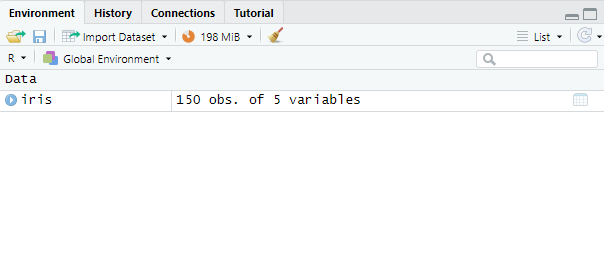
\includegraphics[width=8.39in]{images/environment_forDataDownload}

Si les données sont dans un package, le package doit être importé au préalable.

\subsection{Bases de données issues dans un fichier .RData}\label{bases-de-donnuxe9es-issues-dans-un-fichier-.rdata}

Les fichiers \texttt{.RData} sont spécifique au language R et peuvent contenir plusieurs objets en un seul fichier. Pour importer des données, il faut utiliser la fonction \texttt{load()}

\begin{Shaded}
\begin{Highlighting}[]
\FunctionTok{load}\NormalTok{(}\StringTok{"04{-}data.RData"}\NormalTok{)}
\end{Highlighting}
\end{Shaded}

Tous les objets importés sont chargés dans l'environnement de travail.

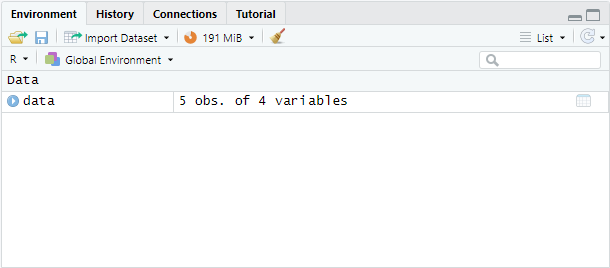
\includegraphics[width=8.47in]{images/environment_forRDataDownload}

\subsection{Bases de données issues de fichiers externes}\label{bases-de-donnuxe9es-issues-de-fichiers-externes}

Les données à analyser sont souvent disponibles dans un fichier externe sous différents formats tels que .csv ou .txt. Pour importer ces données, il existe une fonction par type de fichier (\texttt{read.csv()} et \texttt{read.table()}). Lorsqu'une de ces fonctions est utilisée, le contenu est stocké dans une dataframe. Il est nécessaire de spécifier le chemin d'accès entre votre logiciel et votre fichier à télécharger. Vous pouvez le faire de deux manières:
1. En utilisant la fonction \texttt{setwd()} et en spécifiant à l'intérieur la direction complète qui va permettre au logiciel de retrouver votre document dans vos fichiers.
1. En créant un projet dans lequel vous stockez vos documents.
Ces fonctions acceptent des arguments qui permettent de s'adapter à la nature de fichier à importer. Parmi ces arguments, il y en a trois principaux:

\begin{enumerate}
\def\labelenumi{\arabic{enumi}.}
\tightlist
\item
  \texttt{header} qui est une valeur logique (\texttt{TRUE} ou \texttt{FALSE}) pour la présence d'un en-tête avec les noms de variables. Cet argument est mis par défaut à \texttt{TRUE} pour la fonction \texttt{read.csv()} et à \texttt{FALSE} pour la fonction \texttt{read.table()}.
\item
  \texttt{sep} qui est le caractère dont les champs sont séparés. Cet argument est mis par défaut à \texttt{,}.
\item
  \texttt{dec} qui est le séparateur décimal. Cet argument est mis par défaut à \texttt{.}.
\end{enumerate}

Le seul argument obligatoire est le chemin d'accès au fichier à lire. Il n'est pas nécessaire de spécifier le chemin complet si le fichier à lire se trouve dans le dossier du projet. Si ce n'est pas le cas, vous devez spécifier le chemin d'accès complet à partir de ce qui a été fait avec la fonction \texttt{setwd()}. Pour charger une base de donnée nommé \texttt{04-data.csv} dont les valeurs sont séparées par des virgules, il suffit d'écrire la ligne suivante:

\begin{Shaded}
\begin{Highlighting}[]
\NormalTok{csv\_data }\OtherTok{\textless{}{-}} \FunctionTok{read.csv}\NormalTok{(}\StringTok{"04{-}data.csv"}\NormalTok{)}
\NormalTok{csv\_data}
\end{Highlighting}
\end{Shaded}

\begin{verbatim}
##      Nom Age Note.1 Note.2
## 1   Marc  18    5.0   5.50
## 2   Anne  20    6.0   4.00
## 3 Marie   21    4.5   4.75
## 4   Jean  17    3.5   5.00
## 5 Sophie  18    5.0   4.75
\end{verbatim}

Pour charger une base de donnée nommé \texttt{04-data.txt} dont les valeurs sont séparées par des points-virgules, il suffit d'écrire comme dans la ligne suivante en n'oubliant pas de sécifier le caractère de séparation avec l'argument \texttt{sep=";"}.

\begin{Shaded}
\begin{Highlighting}[]
\NormalTok{txt\_data }\OtherTok{\textless{}{-}} \FunctionTok{read.table}\NormalTok{(}\StringTok{"04{-}data.txt"}\NormalTok{, }\AttributeTok{sep =} \StringTok{";"}\NormalTok{, }\AttributeTok{header =} \ConstantTok{TRUE}\NormalTok{)}
\NormalTok{txt\_data}
\end{Highlighting}
\end{Shaded}

\begin{verbatim}
##      Nom Age Note.1 Note.2
## 1   Marc  18    5.0   5.50
## 2   Anne  20    6.0   4.00
## 3  Marie  21    4.5   4.75
## 4   Jean  17    3.5   5.00
## 5 Sophie  18    5.0   4.75
\end{verbatim}

Il est également possible de charger une base de données issues d'un fichier externe en l'important depuis le menu \texttt{File\ \textgreater{}\ Import\ Dataset\ \textgreater{}\ From\ Text} puis de sélectionner le fichier dans vos dossiers.

\chapter{ANOVA à mesures répétées}\label{anova-uxe0-mesures-ruxe9puxe9tuxe9es}

\section{ANOVA à mesures répétées à un facteur de classification}\label{anova-uxe0-mesures-ruxe9puxe9tuxe9es-uxe0-un-facteur-de-classification}

L'ANOVA à mesures répétées est utilisée lorsque les mêmes sujets sont mesurés plusieurs fois dans différentes conditions ou à différents moments. Pour effectuer l'ANOVA à mesures répétées, nous allons utiliser la fonction \texttt{anova\_test()} du package \texttt{rstatix}. Dans ce chapitre, nous allons traiter de l'ANOVA à mesures répétées avec un et deux facteurs de classification. Nous présentons en détails la question du format, du traitement et de la description des donnés pour l'ANOVA à un facteur de classification. Les mêmes démarches sont à suivre pour l'ANOVA à deux facteurs pour laquelle nous présentons uniquement la marche à suivre de l'ANOVA en tant que telle et son interprétation.

\subsection{Format, traitement et description des données}\label{format-traitement-et-description-des-donnuxe9es}

Afin d'utiliser cette fonction, les données doivent être au format long, à savoir le format dans lequel chaque ligne représente une mesure individuelle avec une colonne identifiant le sujet. La base de données avec laquelle nous travaillons contient trois variables, à savoir \texttt{participants} qui correspond à la variable permettant d'identifier les sujets de l'étude, la variable \texttt{condition} qui correspond aux temps de mesure, et la variable \texttt{score} qui est la variable indépendante mesurée. La variable \texttt{condition} est donc la variable inta-sujet et la variable \texttt{score} la mesure répétée. Dans le traitement des données, il est important de contrôler que la variable des sujets et la variable intra-sujet soient des facteurs, et que la variable à mesures répétées soit numérique. Si ce n'est pas le cas, il est important de les transformer. La fonction \texttt{unique()} permet d'extraire les éléments uniques afin de savoir combien de participants sont présents dans la base de données ou combien de temps de mesure il y a.

\begin{Shaded}
\begin{Highlighting}[]
\FunctionTok{library}\NormalTok{(dplyr) }\CommentTok{\#manipulation des données}
\end{Highlighting}
\end{Shaded}

\begin{verbatim}
## Warning: le package 'dplyr' a été compilé avec la version R 4.3.1
\end{verbatim}

\begin{verbatim}
## 
## Attachement du package : 'dplyr'
\end{verbatim}

\begin{verbatim}
## Les objets suivants sont masqués depuis 'package:stats':
## 
##     filter, lag
\end{verbatim}

\begin{verbatim}
## Les objets suivants sont masqués depuis 'package:base':
## 
##     intersect, setdiff, setequal, union
\end{verbatim}

\begin{Shaded}
\begin{Highlighting}[]
\FunctionTok{library}\NormalTok{(rstatix)}
\end{Highlighting}
\end{Shaded}

\begin{verbatim}
## Warning: le package 'rstatix' a été compilé avec la version R 4.3.3
\end{verbatim}

\begin{verbatim}
## 
## Attachement du package : 'rstatix'
\end{verbatim}

\begin{verbatim}
## L'objet suivant est masqué depuis 'package:stats':
## 
##     filter
\end{verbatim}

\begin{Shaded}
\begin{Highlighting}[]
\NormalTok{data }\OtherTok{\textless{}{-}} \FunctionTok{read.csv}\NormalTok{(}\StringTok{"score.csv"}\NormalTok{, }\AttributeTok{header =} \ConstantTok{TRUE}\NormalTok{, }\AttributeTok{sep =} \StringTok{";"}\NormalTok{, }\AttributeTok{dec =} \StringTok{","}\NormalTok{)}
\FunctionTok{str}\NormalTok{(data)}
\end{Highlighting}
\end{Shaded}

\begin{verbatim}
## 'data.frame':    15 obs. of  3 variables:
##  $ participants: int  1 1 1 2 2 2 3 3 3 4 ...
##  $ condition   : chr  "T1" "T2" "T3" "T1" ...
##  $ score       : num  12.1 14.1 15.3 11.8 13.2 14.7 15.2 16.7 11.7 10.3 ...
\end{verbatim}

\begin{Shaded}
\begin{Highlighting}[]
\NormalTok{data}\SpecialCharTok{$}\NormalTok{participants }\OtherTok{\textless{}{-}} \FunctionTok{as.factor}\NormalTok{(data}\SpecialCharTok{$}\NormalTok{participants)}
\NormalTok{data}\SpecialCharTok{$}\NormalTok{condition }\OtherTok{\textless{}{-}} \FunctionTok{as.factor}\NormalTok{(data}\SpecialCharTok{$}\NormalTok{condition)}
\FunctionTok{str}\NormalTok{(data)}
\end{Highlighting}
\end{Shaded}

\begin{verbatim}
## 'data.frame':    15 obs. of  3 variables:
##  $ participants: Factor w/ 5 levels "1","2","3","4",..: 1 1 1 2 2 2 3 3 3 4 ...
##  $ condition   : Factor w/ 3 levels "T1","T2","T3": 1 2 3 1 2 3 1 2 3 1 ...
##  $ score       : num  12.1 14.1 15.3 11.8 13.2 14.7 15.2 16.7 11.7 10.3 ...
\end{verbatim}

\begin{Shaded}
\begin{Highlighting}[]
\FunctionTok{unique}\NormalTok{(data}\SpecialCharTok{$}\NormalTok{participants)}
\end{Highlighting}
\end{Shaded}

\begin{verbatim}
## [1] 1 2 3 4 5
## Levels: 1 2 3 4 5
\end{verbatim}

\begin{Shaded}
\begin{Highlighting}[]
\FunctionTok{unique}\NormalTok{(data}\SpecialCharTok{$}\NormalTok{condition)}
\end{Highlighting}
\end{Shaded}

\begin{verbatim}
## [1] T1 T2 T3
## Levels: T1 T2 T3
\end{verbatim}

\subsection{Effectuer et interpréter l'ANOVA}\label{effectuer-et-interpruxe9ter-lanova}

L'ANOVA s'effectue grâce à la fonction \texttt{anova\_test()} en utilisant les arguments suivants:

\begin{enumerate}
\def\labelenumi{\arabic{enumi}.}
\tightlist
\item
  \textbf{dv}: variable dépendante numérique
\item
  \textbf{within}: variable intra-sujet sous forme de facteur
\item
  \textbf{wid}: variable sous forme de facteur permettant d'identifier les sujets
\end{enumerate}

Afin de pouvoir interpréter une ANOVA, des hypothèses doivent être vérifiées. Il s'agit de l'hypothèse de normalité des données, que l'on teste grâce à la fonction \texttt{shapiro\_test()} avant d'effectuer l'ANOVA, et l'hypothèse de sphérécité des données, que l'on contrôle directement dans le résultat de l'ANOVA.

L'hypothèse nulle du test de la normalité des données est que les données suivent une loi normale. Si cette hypothèse n'est pas rejetée, alors l'ANOVA à mesures répétées peut être effectuée. L'hypothèse nulle du test de sphérécité considère l'égalité des variances des différences des groupes. Si l'hypothèse nulle n'est pas rejetée, alors aucune correction est nécessaire. Au contraire, une correction doit s'appliquer.

La fonction \texttt{get\_anova\_table()} permet d'obtenir le résultat de l'ANOVA. Nous proposons d'utiliser l'argument \texttt{correction\ =\ "auto"} car il permet d'effectuer la correction nécessaire si l'hypothèse de sphérécité des données est rejetée.

\begin{Shaded}
\begin{Highlighting}[]
\NormalTok{data }\SpecialCharTok{\%\textgreater{}\%}
  \FunctionTok{group\_by}\NormalTok{(condition) }\SpecialCharTok{\%\textgreater{}\%}
  \FunctionTok{shapiro\_test}\NormalTok{(score)}
\end{Highlighting}
\end{Shaded}

\begin{verbatim}
## # A tibble: 3 x 4
##   condition variable statistic     p
##   <fct>     <chr>        <dbl> <dbl>
## 1 T1        score        0.973 0.894
## 2 T2        score        0.969 0.872
## 3 T3        score        0.896 0.386
\end{verbatim}

\begin{Shaded}
\begin{Highlighting}[]
\NormalTok{res }\OtherTok{\textless{}{-}} \FunctionTok{anova\_test}\NormalTok{(data, }\AttributeTok{dv =}\NormalTok{ score, }\AttributeTok{within =}\NormalTok{ condition, }\AttributeTok{wid =}\NormalTok{ participants)}

\FunctionTok{print}\NormalTok{(res}\SpecialCharTok{$}\StringTok{\textasciigrave{}}\AttributeTok{Mauchly\textquotesingle{}s Test for Sphericity}\StringTok{\textasciigrave{}}\NormalTok{)}
\end{Highlighting}
\end{Shaded}

\begin{verbatim}
##      Effect     W     p p<.05
## 1 condition 0.876 0.819
\end{verbatim}

\begin{Shaded}
\begin{Highlighting}[]
\NormalTok{res }\SpecialCharTok{\%\textgreater{}\%} \FunctionTok{get\_anova\_table}\NormalTok{()}
\end{Highlighting}
\end{Shaded}

\begin{verbatim}
## ANOVA Table (type III tests)
## 
##      Effect DFn DFd     F     p p<.05   ges
## 1 condition   2   8 0.446 0.655       0.077
\end{verbatim}

\begin{Shaded}
\begin{Highlighting}[]
\NormalTok{res }\SpecialCharTok{\%\textgreater{}\%} \FunctionTok{get\_anova\_table}\NormalTok{(}\AttributeTok{correction =} \StringTok{"auto"}\NormalTok{)}
\end{Highlighting}
\end{Shaded}

\begin{verbatim}
## ANOVA Table (type III tests)
## 
##      Effect DFn DFd     F     p p<.05   ges
## 1 condition   2   8 0.446 0.655       0.077
\end{verbatim}

Enfin d'interpréter le résultat de l'ANOVA, il est nécessaire d'analyser la table de l'ANOVA:

\begin{enumerate}
\def\labelenumi{\arabic{enumi}.}
\tightlist
\item
  \textbf{Effet}: la variable intra-sujet
\item
  \textbf{DFn}: degrés de liberté du facteur intra-sujet
\item
  \textbf{DFd}: degrés de liberté de l'erreur intra-sujet
\item
  \textbf{F}: statistique F de Fisher
\item
  \textbf{p}: significativité du test
\item
  \textbf{ges}: taille de l'effet généralisée aussi appelée êta carré
\end{enumerate}

La significativité du test permet de conclure sur la présence ou l'absence d'un effet significatif de la condition sur le score, donc de l'impact des temps de mesure sur le score. La taille d'effet permet d'évaluer l'importance de l'effet. Elle doit être analysée selon la grille d'analyse correspondante.

\subsection{Test post-hoc}\label{test-post-hoc}

Si l'ANOVA est significative, il est important d'effectuer un test post-hoc pour savoir quelles conditions diffèrent. Le test post-hoc est effectué avec la fonction \texttt{pairwise\_t\_test()} pour comparer les données pair à pair avec une correction de Bonferroni. L'interprétation se fait comme dans le cas d'un test de Student à mesures répétées.

\begin{Shaded}
\begin{Highlighting}[]
\FunctionTok{pairwise\_t\_test}\NormalTok{(data, score }\SpecialCharTok{\textasciitilde{}}\NormalTok{ condition, }\AttributeTok{paired =} \ConstantTok{TRUE}\NormalTok{, }
                \AttributeTok{p.adjust.method =} \StringTok{"bonferroni"}\NormalTok{)}
\end{Highlighting}
\end{Shaded}

\begin{verbatim}
## # A tibble: 3 x 10
##   .y.   group1 group2    n1    n2 statistic    df     p p.adj p.adj.signif
## * <chr> <chr>  <chr>  <int> <int>     <dbl> <dbl> <dbl> <dbl> <chr>       
## 1 score T1     T2         5     5    -1.06      4 0.347     1 ns          
## 2 score T1     T3         5     5    -0.472     4 0.661     1 ns          
## 3 score T2     T3         5     5     0.419     4 0.697     1 ns
\end{verbatim}

\section{ANOVA à mesures répétées à deux facteurs de classification}\label{anova-uxe0-mesures-ruxe9puxe9tuxe9es-uxe0-deux-facteurs-de-classification}

\subsection{Données}\label{donnuxe9es}

Les mêmes manipulations préalables que pour l'ANOVA à mesures répétées avec un facteur de classification sont à effectuer. La base de données avec laquelle on travaille contient des scores répétés à trois reprises pour dix individus qui sont répartis dans deux groupes, soit expérimental, soit contrôle.

\begin{Shaded}
\begin{Highlighting}[]
\NormalTok{data }\OtherTok{\textless{}{-}} \FunctionTok{read.csv}\NormalTok{(}\StringTok{"diet.csv"}\NormalTok{)}

\FunctionTok{str}\NormalTok{(data)}
\end{Highlighting}
\end{Shaded}

\begin{verbatim}
## 'data.frame':    72 obs. of  4 variables:
##  $ id       : int  1 2 3 4 5 6 7 8 9 10 ...
##  $ treatment: chr  "ctr" "ctr" "ctr" "ctr" ...
##  $ time     : chr  "t1" "t1" "t1" "t1" ...
##  $ score    : int  83 97 93 92 77 72 92 92 95 92 ...
\end{verbatim}

\begin{Shaded}
\begin{Highlighting}[]
\NormalTok{data }\OtherTok{\textless{}{-}}\NormalTok{ data }\SpecialCharTok{\%\textgreater{}\%}
  \FunctionTok{mutate}\NormalTok{(}\AttributeTok{id =} \FunctionTok{as.factor}\NormalTok{(id),}
         \AttributeTok{treatment =} \FunctionTok{as.factor}\NormalTok{(treatment),}
         \AttributeTok{time =} \FunctionTok{as.factor}\NormalTok{(time), }
         \AttributeTok{score =} \FunctionTok{as.numeric}\NormalTok{(score))}

\FunctionTok{str}\NormalTok{(data)}
\end{Highlighting}
\end{Shaded}

\begin{verbatim}
## 'data.frame':    72 obs. of  4 variables:
##  $ id       : Factor w/ 12 levels "1","2","3","4",..: 1 2 3 4 5 6 7 8 9 10 ...
##  $ treatment: Factor w/ 2 levels "ctr","Diet": 1 1 1 1 1 1 1 1 1 1 ...
##  $ time     : Factor w/ 3 levels "t1","t2","t3": 1 1 1 1 1 1 1 1 1 1 ...
##  $ score    : num  83 97 93 92 77 72 92 92 95 92 ...
\end{verbatim}

\begin{Shaded}
\begin{Highlighting}[]
\FunctionTok{unique}\NormalTok{(data}\SpecialCharTok{$}\NormalTok{id)}
\end{Highlighting}
\end{Shaded}

\begin{verbatim}
##  [1] 1  2  3  4  5  6  7  8  9  10 11 12
## Levels: 1 2 3 4 5 6 7 8 9 10 11 12
\end{verbatim}

\begin{Shaded}
\begin{Highlighting}[]
\FunctionTok{unique}\NormalTok{(data}\SpecialCharTok{$}\NormalTok{time)}
\end{Highlighting}
\end{Shaded}

\begin{verbatim}
## [1] t1 t2 t3
## Levels: t1 t2 t3
\end{verbatim}

\begin{Shaded}
\begin{Highlighting}[]
\FunctionTok{unique}\NormalTok{(data}\SpecialCharTok{$}\NormalTok{treatment)}
\end{Highlighting}
\end{Shaded}

\begin{verbatim}
## [1] ctr  Diet
## Levels: ctr Diet
\end{verbatim}

\subsection{ANOVA}\label{anova}

La présence de deux facteurs de classification change l'argument \texttt{within} de la fonction \texttt{anova\_test()}. En effet, il n'y a plus une mais deux variable intra-sujet. Dans le tableau de l'ANOVA à mesures répétées avec deux facteurs de classification, il y a trois effets:

\begin{enumerate}
\def\labelenumi{\arabic{enumi}.}
\tightlist
\item
  L'effet principal du facteur temps qui teste si les scores changent significativement entre les trois temps de mesure. L'hypothèse nulle est l'absence de différence entre les temps.
\item
  L'effet principal du groupe qui test si l'appartenance à un groupe influence significativement le score. L'hypothèse nulle est l'absence de différence entre les groupes.
\item
  L'interaction entre les deux facteurs intra-sujet qui teste si l'évolution des scores dans le temps diffère selon le groupe d'appartenance. L'hypothèse nulle stipule qu'il n'y a pas d'interaction entre les deux facteurs
\end{enumerate}

\begin{Shaded}
\begin{Highlighting}[]
\NormalTok{data }\SpecialCharTok{\%\textgreater{}\%}
  \FunctionTok{group\_by}\NormalTok{(time, treatment) }\SpecialCharTok{\%\textgreater{}\%}
  \FunctionTok{shapiro\_test}\NormalTok{(score)}
\end{Highlighting}
\end{Shaded}

\begin{verbatim}
## # A tibble: 6 x 5
##   treatment time  variable statistic      p
##   <fct>     <fct> <chr>        <dbl>  <dbl>
## 1 ctr       t1    score        0.828 0.0200
## 2 Diet      t1    score        0.919 0.279 
## 3 ctr       t2    score        0.868 0.0618
## 4 Diet      t2    score        0.923 0.316 
## 5 ctr       t3    score        0.887 0.107 
## 6 Diet      t3    score        0.886 0.104
\end{verbatim}

\begin{Shaded}
\begin{Highlighting}[]
\NormalTok{res }\OtherTok{\textless{}{-}}\NormalTok{  data }\SpecialCharTok{\%\textgreater{}\%}
  \FunctionTok{anova\_test}\NormalTok{(}\AttributeTok{dv =}\NormalTok{ score, }\AttributeTok{wid =}\NormalTok{ id, }\AttributeTok{within =} \FunctionTok{c}\NormalTok{(time, treatment))}

\FunctionTok{print}\NormalTok{(res}\SpecialCharTok{$}\StringTok{\textasciigrave{}}\AttributeTok{Mauchly\textquotesingle{}s Test for Sphericity}\StringTok{\textasciigrave{}}\NormalTok{)}
\end{Highlighting}
\end{Shaded}

\begin{verbatim}
##           Effect     W     p p<.05
## 1           time 0.469 0.023     *
## 2 time:treatment 0.616 0.089
\end{verbatim}

\begin{Shaded}
\begin{Highlighting}[]
\NormalTok{res }\SpecialCharTok{\%\textgreater{}\%} \FunctionTok{get\_anova\_table}\NormalTok{(}\AttributeTok{correction =} \StringTok{"auto"}\NormalTok{)}
\end{Highlighting}
\end{Shaded}

\begin{verbatim}
## ANOVA Table (type III tests)
## 
##           Effect  DFn   DFd      F        p p<.05   ges
## 1           time 1.31 14.37 27.369 5.03e-05     * 0.049
## 2      treatment 1.00 11.00 15.541 2.00e-03     * 0.059
## 3 time:treatment 2.00 22.00 30.424 4.63e-07     * 0.050
\end{verbatim}

Dans notre cas, on observe que les deux facteurs sont significatifs, tout comme l'interaction entre eux. Comme l'interactione est significative, il est nécessaire de poursuivre l'analyse en effectuant une ANOVA à mesures répétées à un facteur pour la première variable pour chaque niveau de la deuxième variable, puis de faire des comparaisons multiples si l'ANOVA est significative.

Si l'interaction devait ne pas être significative, il est nécessaire de faire l'analyse des effets principaux directement.

  \bibliography{book.bib,packages.bib}

\end{document}
